% Provenance (never printed): see sources/outline_sources.md (Year 3:
% dislocation and diffusion creep; flow laws; deformation maps; shear zones and
% kinematic indicators). Brief: sources/book5/BRIEFS.md, ch. 7. Curves from
% figdata/bachelor-3/flow_laws.py. Exercise and problem values in the Book 5
% scratch calculator calc/ch07.py.
\chapter{Mecanismos de deformación y zonas de cizalla}\label{ch:b3:deformation-mechanisms}

En superficie, el granito de una montaña se fractura a lo largo de fallas.
A veinte kilómetros de profundidad, el mismo granito fluye como un caramelo blando en una \omterm{def:b3:deformation-mechanisms:shear-zone}{zona de cizalla} de unos
cientos de metros de ancho, sus feldespatos se redondean en forma de ojos y su cuarzo se alarga
en cintas. Un cristal puede fluir sin romperse porque nunca es perfecto:
se desplaza gracias a sus defectos, una fila de átomos cada vez, o por la difusión de átomos desde
una cara de un grano hacia otra. Este capítulo recorre esos mecanismos desde la
red cristalina hasta las leyes que emplea la geodinámica, hasta los mapas que indican qué
mecanismo domina, y hasta las \omterm{def:b3:deformation-mechanisms:shear-zone}{zonas de cizalla} en las que la roca registra cómo se movió.

\begin{recall}
Los defectos puntuales, la ley de Arrhenius y la energía de activación se tratan en los
volúmenes universitarios de los libros de química; el coeficiente de difusión, en los de
física. Esfuerzo y deformación, la elipse de deformación, la cizalla simple y su elipse
($S_{1,2} = \sqrt{1 + \gamma^2/4} \pm \gamma/2$, eje largo a $\theta'$ de la
dirección de cizalla con $\tan2\theta' = 2/\gamma$), la fluencia de ley potencial con sus
constantes para la cuarcita húmeda y el olivino seco, la envolvente de resistencia y la
transición frágil--dúctil se tratan en el volumen de primer año, en su capítulo sobre
esfuerzo, deformación y reología; la foliación, la lineación y la
milonita descriptiva, en su capítulo sobre fallas, pliegues y fábricas. La viscosidad efectiva
del manto se encuentra en el \cref{ch:b3:mantle-convection}.
\end{recall}

\section{Defectos cristalinos}

Para cizallar un cristal perfecto, cada enlace a través de un plano reticular tendría que
romperse a la vez, y eso exige un esfuerzo del orden de una décima parte del módulo de
cizalla, que en el manto es de unos \qty{8e10}{Pa}
(el \cref{ch:b3:mantle-convection}): miles de megapascales. Los cristales reales
ceden con esfuerzos mucho menores, porque deslizan una línea de átomos cada vez.

\begin{definition}[Dislocación]\label{def:b3:deformation-mechanisms:dislocation}
Una \emph{dislocación}\index{dislocación (defecto cristalino)} es un defecto lineal en un
cristal: la frontera, dentro del cristal, entre una parte de un plano reticular
que ha deslizado y una parte que no. Su \emph{vector de Burgers}
$\mathbf b$ es el deslizamiento que transporta, una distancia reticular en una
dirección reticular. En una dislocación de borde $\mathbf b$ es perpendicular a la línea,
que es el borde de un semiplano extra de átomos; en una dislocación helicoidal es
paralela a la línea. Una dislocación se desplaza por \emph{deslizamiento conservativo} en su plano de deslizamiento,
y una dislocación de borde abandona ese plano por \emph{trepado}, al difundirse átomos o
vacantes hacia el borde de su semiplano o desde él.
\end{definition}

\begin{omfigure}
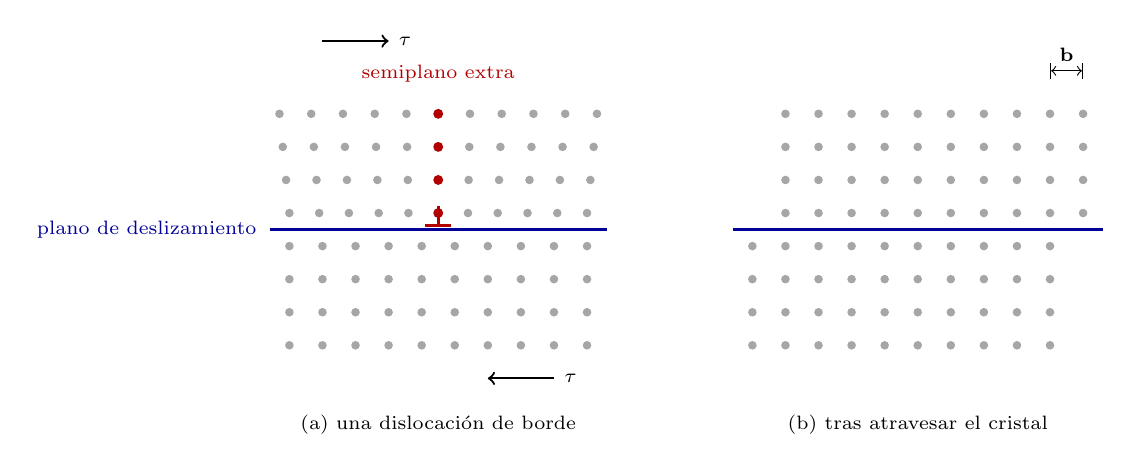
\begin{tikzpicture}[font=\scriptsize, x=0.42cm, y=0.42cm]
% (a) lower half: 10 columns; upper half: 11 columns squeezed over the same width
\foreach \j in {0,...,3} {\foreach \i in {0,...,9} {\fill[gray!70] (\i,\j) circle (0.13);}}
\foreach \j/\s in {4/0.9, 5/0.92, 6/0.94, 7/0.96} {\foreach \i in {0,...,10} {
  \pgfmathsetmacro{\x}{(\i-5)*\s + 4.5}
  \ifnum\i=5 \fill[red!70!black] (\x,\j) circle (0.15); \else \fill[gray!70] (\x,\j) circle (0.13); \fi}}
\draw[thick, blue!60!black] (-0.6,3.5) -- (9.6,3.5);
 \node[anchor=east, blue!60!black] at (-0.7,3.5) {plano de deslizamiento};
\draw[red!70!black, very thick] (4.1,3.62) -- (4.9,3.62) (4.5,3.62) -- (4.5,4.2);
 \node[red!70!black] at (4.5,8.2) {semiplano extra};
\draw[->, thick] (1.0,9.2) -- (3.0,9.2) node[right] {$\tau$};
\draw[<-, thick] (6.0,-1.0) -- (8.0,-1.0) node[right] {$\tau$};
% (b) after glide: the upper half shifted by one spacing
\begin{scope}[shift={(14,0)}]
\foreach \j in {0,...,3} {\foreach \i in {0,...,9} {\fill[gray!70] (\i,\j) circle (0.13);}}
\foreach \j in {4,...,7} {\foreach \i in {1,...,10} {\fill[gray!70] (\i,\j) circle (0.13);}}
\draw[thick, blue!60!black] (-0.6,3.5) -- (10.6,3.5);
\draw[|<->|] (9,8.3) -- (10,8.3) node[midway, above] {$\mathbf b$};
\end{scope}
 \node[anchor=north] at (4.5,-1.8) {(a) una dislocación de borde};
 \node[anchor=north] at (19,-1.8) {(b) tras atravesar el cristal};
\end{tikzpicture}

\par\smallskip{\small (a) Una \omterm{def:b3:deformation-mechanisms:dislocation}{dislocación} de borde: un semiplano extra de átomos (en rojo)
termina en el plano de deslizamiento, distorsionando la red alrededor de su borde (el símbolo
$\perp$). Bajo el esfuerzo de cizalla $\tau$ se desplaza a lo largo del plano de deslizamiento al
romper y reformar una fila de enlaces cada vez. (b) Cuando ha atravesado el
cristal, la mitad superior ha deslizado un vector de Burgers $\mathbf b$, y la
red vuelve a ser perfecta.}\label{fig:b3:deformation-mechanisms:dislocation}
\end{omfigure}

La red se opone al deslizamiento conservativo de una \omterm{def:b3:deformation-mechanisms:dislocation}{dislocación} con un esfuerzo pequeño, el
esfuerzo de Peierls, que depende de la intensidad y de la dirección de los enlaces:
por eso algunos sistemas de deslizamiento de un mineral son fáciles y otros difíciles. A medida que
un cristal se deforma, las dislocaciones se multiplican y se enredan; se bloquean unas a otras, y
el cristal se endurece, salvo que puedan trepar alrededor de los obstáculos o aniquilarse, lo que
requiere difusión y, por tanto, calor.

\section{Mecanismos de fluencia}

\begin{definition}[Mecanismos de fluencia]\label{def:b3:deformation-mechanisms:creep}
En la \emph{fluencia por dislocaciones}\index{fluencia por dislocaciones} los cristales se deforman por el
deslizamiento conservativo de las dislocaciones, y el trepado las libera de los obstáculos. En la
\emph{fluencia por difusión}\index{fluencia por difusión} cambian de forma por la
difusión de átomos, a través de la red (fluencia de Nabarro--Herring) o a lo largo de los
bordes de grano (fluencia de Coble), desde las caras sometidas al mayor esfuerzo normal
hacia las sometidas al menor. En el \emph{deslizamiento en borde de grano}\index{deslizamiento en borde de grano}
los granos se deslizan unos junto a otros a lo largo de sus bordes, y los huecos se
cierran por difusión o fluencia por dislocaciones. En la \emph{disolución por
presión}\index{disolución por presión} la materia se disuelve en una película fluida en las
caras sometidas a esfuerzo alto y se deposita donde el esfuerzo es bajo, o se transporta
a otro lugar.
\end{definition}

\begin{proposition}[Dependencia del tamaño de grano en la fluencia por difusión]\label{prop:b3:deformation-mechanisms:grain-size}
Con esfuerzo bajo $\sigma$, una roca de tamaño de grano $d$ fluye por difusión a la velocidad
\[
  \dot\varepsilon \approx B_L\frac{D_L\Omega}{k_BT}\frac{\sigma}{d^2}
  \quad\text{(a través de la red)},\qquad
  \dot\varepsilon \approx B_B\frac{\delta D_B\Omega}{k_BT}\frac{\sigma}{d^3}
  \quad\text{(a lo largo de los bordes)},
\]
donde $D_L$ y $D_B$ son los coeficientes de difusión en la red y en los
bordes, $\delta$ el ancho de un borde, $\Omega$ el volumen de un átomo,
$k_B$ la constante de Boltzmann y $B_L$, $B_B$ números del orden de diez que dependen de
la forma de los granos.
\end{proposition}

\begin{proof}
Un esfuerzo normal $\sigma$ sobre una cara modifica el trabajo necesario para formar una vacante
allí en $\sigma\Omega$, de modo que la concentración $C$ de vacantes difiere entre
las caras sometidas a tracción y las sometidas a compresión en $\Delta C \approx C\sigma\Omega/
(k_BT)$ cuando $\sigma\Omega \ll k_BT$. A través de una distancia del orden de $d$, el
flujo difusivo de vacantes, y por tanto de átomos en sentido contrario, es del orden de $D\Delta
C/d$ por unidad de área. A través de la red, el flujo atraviesa un área del orden de
$d^2$; a lo largo de los bordes, un área del orden de $\delta d$. El volumen desplazado por
unidad de tiempo, dividido por el volumen del grano $d^3$, es la velocidad de deformación: del orden de
$(D_L\sigma\Omega/k_BT)\,d^2/(d\cdot d^3) = D_L\sigma\Omega/(k_BTd^2)$ en la
red, y $(D_B\sigma\Omega/k_BT)\,\delta d/(d\cdot d^3) = \delta D_B
\sigma\Omega/(k_BTd^3)$ en los bordes. El producto $C\,D$ es el
coeficiente de autodifusión que en el enunciado se escribe $D$.
\end{proof}

La \omterm{def:b3:deformation-mechanisms:creep}{fluencia por difusión} es lineal en el esfuerzo, un auténtico flujo viscoso, y es rápida en
rocas de grano fino: al reducir a la mitad el tamaño de grano, la fluencia de Coble se vuelve
ocho veces más rápida (figura siguiente). La \omterm{def:b3:deformation-mechanisms:creep}{fluencia por dislocaciones} no depende del tamaño
de grano, pero crece con una potencia elevada del esfuerzo.

\begin{omfigure}
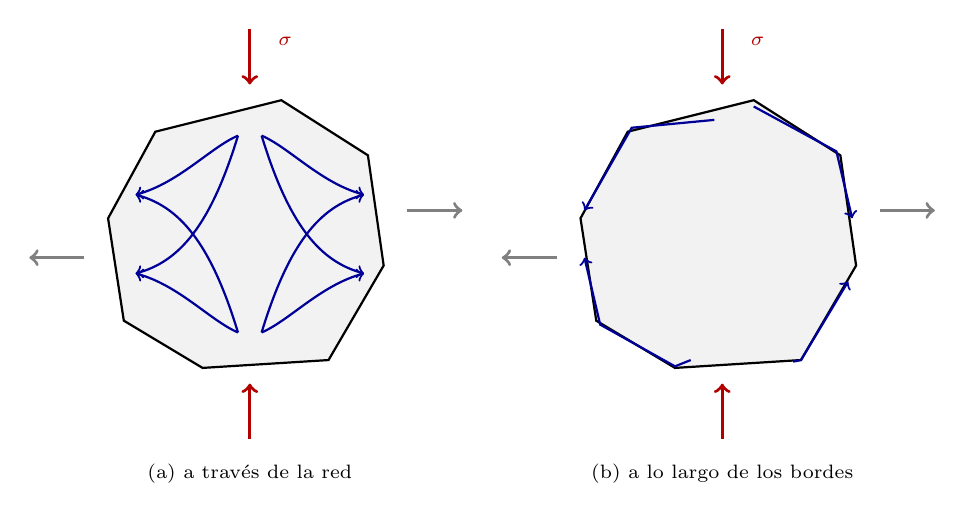
\begin{tikzpicture}[font=\scriptsize, x=1cm, y=1cm]
\foreach \cx/\lab in {0/{(a) a través de la red}, 6/{(b) a lo largo de los bordes}} {
  \begin{scope}[shift={(\cx,0)}]
  \draw[thick, fill=gray!10] (-1.6,-1.1) -- (-0.6,-1.7) -- (1.0,-1.6) -- (1.7,-0.4) -- (1.5,1.0) -- (0.4,1.7) -- (-1.2,1.3) -- (-1.8,0.2) -- cycle;
  \draw[->, very thick, red!70!black] (0,2.6) -- (0,1.9);
  \draw[->, very thick, red!70!black] (0,-2.6) -- (0,-1.9);
  \node[red!70!black] at (0.45,2.45) {$\sigma$};
  \draw[<-, very thick, gray] (2.7,0.3) -- (2.0,0.3);
  \draw[<-, very thick, gray] (-2.8,-0.3) -- (-2.1,-0.3);
  \node[anchor=north] at (0,-2.8) {\lab};
  \end{scope}
}
\foreach \sx in {1,-1} {\foreach \y in {-0.5,0.5} {
  \draw[->, blue!60!black, thick] (0.15*\sx,1.25) .. controls (0.5*\sx,\y+0.6) and (0.9*\sx,\y+0.15) .. (1.45*\sx,\y);
  \draw[->, blue!60!black, thick] (0.15*\sx,-1.25) .. controls (0.5*\sx,\y-0.6) and (0.9*\sx,\y-0.15) .. (1.45*\sx,\y);
}}
\draw[->, blue!60!black, thick] (6.4,1.62) -- (7.45,1.05) -- (7.65,0.2);
\draw[->, blue!60!black, thick] (5.9,1.45) -- (4.85,1.35) -- (4.25,0.3);
\draw[->, blue!60!black, thick] (6.9,-1.62) -- (7.0,-1.6) -- (7.6,-0.6);
\draw[->, blue!60!black, thick] (5.6,-1.6) -- (5.4,-1.68) -- (4.45,-1.15) -- (4.25,-0.3);
\end{tikzpicture}

\par\smallskip{\small \omterm{def:b3:deformation-mechanisms:creep}{Fluencia por difusión} de un grano acortado a lo largo de $\sigma$. Los átomos
abandonan las caras bajo la compresión más alta y se añaden a las caras bajo la
menor (azul), de modo que el grano se aplana y se alarga (flechas grises): (a)
a través del interior del grano, fluencia de Nabarro--Herring; (b) a lo largo de sus bordes,
fluencia de Coble.}\label{fig:b3:deformation-mechanisms:diffusion}
\end{omfigure}

Los cristales deformados también se reparan mientras se deforman.

\begin{definition}[Recuperación, subgrano, recristalización dinámica]\label{def:b3:deformation-mechanisms:recrystallisation}
La \emph{recuperación}\index{recuperación (plasticidad cristalina)} es la reordenación de
dislocaciones, por trepado y deslizamiento cruzado, en configuraciones de menor energía, y su
aniquilación. Las dislocaciones dispuestas en paredes dividen un grano en
\emph{subgranos}\index{subgrano}, partes del grano cuyas redes están inclinadas
unos pocos grados entre sí. La \emph{recristalización
dinámica}\index{recristalización dinámica} es el reemplazo, durante
la deformación, de granos deformados por nuevos granos con menos dislocaciones, bien
por la rotación de subgranos hasta convertirse en granos, bien por la migración de
los bordes de grano hacia los vecinos más deformados.
\end{definition}

\begin{definition}[Orientación cristalográfica preferente]\label{def:b3:deformation-mechanisms:cpo}
Una roca tiene una \emph{orientación cristalográfica preferente}\index{orientación cristalográfica preferente}
(CPO) cuando las redes de sus granos no están orientadas
al azar, sino que se agrupan en torno a direcciones fijadas por la deformación; la \omterm{def:b3:deformation-mechanisms:creep}{fluencia
por dislocaciones} la produce, al girar los sistemas de deslizamiento de cada grano hacia el flujo.
\end{definition}

Una roca con CPO hereda la anisotropía de sus cristales: sus velocidades sísmicas,
por ejemplo, dependen de la dirección, lo que permite a la sismología ver la fábrica del
manto profundo. La \omterm{def:b3:deformation-mechanisms:creep}{fluencia por difusión} y el \omterm{def:b3:deformation-mechanisms:creep}{deslizamiento en borde de grano}, que dejan girar
libremente a los granos, no la construyen.

\section{Leyes de flujo}

\begin{definition}[Ley de flujo, exponente de esfuerzo, temperatura homóloga]\label{def:b3:deformation-mechanisms:flow-law}
Una \emph{ley de flujo}\index{ley de flujo} da la velocidad de deformación de una roca que se deforma
por un único mecanismo en función del esfuerzo diferencial $\sigma$, el tamaño de grano
$d$, la temperatura $T$ y la presión $P$:
\[
  \dot\varepsilon = A\,\sigma^nd^{-m}\exp\Bigl(-\frac{E + PV}{RT}\Bigr),
\]
con $A$, $n$, $m$, la energía de activación $E$ y el volumen de activación $V$
medidos en el laboratorio. El \emph{exponente de esfuerzo}\index{exponente de esfuerzo}
es $n$; el exponente del tamaño de grano, $m$. La \emph{temperatura
homóloga}\index{temperatura homóloga} de un mineral es $T/T_m$, su temperatura absoluta
dividida por su temperatura absoluta de fusión.
\end{definition}

En las leyes empleadas aquí, la \omterm{def:b3:deformation-mechanisms:creep}{fluencia por dislocaciones} tiene $n$ de 3.5 o 4 y $m = 0$;
la \omterm{def:b3:deformation-mechanisms:creep}{fluencia por difusión} tiene $n = 1$ y $m = 2$ o 3 (\cref{prop:b3:deformation-mechanisms:grain-size}).
La fluencia crece a medida que la \omterm{def:b3:deformation-mechanisms:flow-law}{temperatura homóloga} se acerca a 1. La forsterita funde a \qty{1890}{\celsius}, así que el manto a \qty{1300}{\celsius}
se encuentra en $T/T_m = 0.73$; el hielo a \qty{-10}{\celsius} está en 0.96, por lo que
los glaciares fluyen. Los valores del olivino empleados aquí son los de una compilación
de laboratorio muy utilizada: olivino seco en \omterm{def:b3:deformation-mechanisms:creep}{fluencia por dislocaciones}, $A =
\num{1.1e5}$, $n = 3.5$, $E = \qty{530}{kJ.mol^{-1}}$, $V =
\qty{14}{cm^3.mol^{-1}}$; en \omterm{def:b3:deformation-mechanisms:creep}{fluencia por difusión}, $A = 10^{9.2}$, $n = 1$, $m = 3$,
$E = \qty{375}{kJ.mol^{-1}}$, $V = \qty{5}{cm^3.mol^{-1}}$ (esfuerzo en megapascales,
tamaño de grano en micrómetros, tiempo en segundos); la cuarcita húmeda es la del volumen
de primer año. El agua debilita el olivino: a una fugacidad de agua de unos
\qty{300}{MPa}, los agregados de olivino se deforman entre cinco y seis veces más rápido que los secos
en \omterm{def:b3:deformation-mechanisms:creep}{fluencia por dislocaciones}, y cinco veces más rápido en \omterm{def:b3:deformation-mechanisms:creep}{fluencia por difusión}.
% ledger: bowen14:mgo-sio2, azuma17:olivine, lopez:flow-laws, codata:R, mk00:diffusion, mk00:dislocation

\begin{proposition}[Viscosidad efectiva]\label{prop:b3:deformation-mechanisms:viscosity}
Una roca que obedece una \omterm{def:b3:deformation-mechanisms:flow-law}{ley de flujo} $\dot\varepsilon = A'\sigma^n$ a $T$, $P$ y
$d$ dados tiene la viscosidad efectiva
\[
  \eta_{\mathrm{eff}} = \frac{\sigma}{2\dot\varepsilon}
  = \tfrac12A'^{-1/n}\,\dot\varepsilon^{(1-n)/n}:
\]
para $n > 1$ la viscosidad disminuye a medida que la roca se deforma más rápido.
\end{proposition}

\begin{proof}
Para un fluido newtoniano, $\sigma = 2\eta\dot\varepsilon$ en un flujo uniaxial, por la
definición de viscosidad; $\eta_{\mathrm{eff}}$ es la viscosidad del fluido newtoniano
que fluiría a la misma velocidad de deformación bajo el mismo esfuerzo. Sustituyendo
$\sigma = (\dot\varepsilon/A')^{1/n}$ se obtiene la segunda forma.
\end{proof}

Cuarcita húmeda a \qty{400}{\celsius} que fluye a \qty{e-14}{s^{-1}} necesita
\qty{65}{MPa} y tiene una viscosidad efectiva de \qty{3.3e21}{Pa.s}; a
\qty{500}{\celsius}, \qty{18}{MPa} y \qty{9e20}{Pa.s}: cien grados
dividen la resistencia por más de tres (figura siguiente). La olivina seca a
\qty{1100}{\celsius} y \qty{1}{GPa} necesita solo \qty{3}{MPa}. Las envolventes de resistencia
del volumen de primer año se construyen precisamente a partir de estas leyes.

\begin{omfigure}
\begin{tikzpicture}
\begin{groupplot}[group style={group size=2 by 1, horizontal sep=1.6cm},
  omrecord, width=0.47\linewidth, height=0.47\linewidth, xmode=log,
  xmin=1, xmax=1000, ymin=-20, ymax=-6, xlabel={esfuerzo diferencial (MPa)},
  legend style={font=\scriptsize, at={(0.97,0.03)}, anchor=south east, legend columns=1}]
\nextgroupplot[ylabel={$\log_{10}\dot\varepsilon$ (\unit{s^{-1}})}, title={(a) cuarcita húmeda},
  title style={font=\small}]
% computed in figdata/bachelor-3/flow_laws.py; ledger: lopez:flow-laws, azuma17:olivine
\addplot[omDef, thick] table[x=s, y=r600] {figdata/out/bachelor-3-flow_laws-quartz.dat};
\addlegendentry{\qty{600}{\celsius}}
\addplot[red!70!black, thick, densely dashed] table[x=s, y=r500] {figdata/out/bachelor-3-flow_laws-quartz.dat};
\addlegendentry{\qty{500}{\celsius}}
\addplot[black, thick, densely dotted] table[x=s, y=r400] {figdata/out/bachelor-3-flow_laws-quartz.dat};
\addlegendentry{\qty{400}{\celsius}}
\draw[gray] (axis cs:1,-14) -- (axis cs:1000,-14);
\nextgroupplot[title={(b) olivina seca, \qty{1}{GPa}}, title style={font=\small}]
\addplot[omDef, thick] table[x=s, y=r1300] {figdata/out/bachelor-3-flow_laws-olivine.dat};
\addlegendentry{\qty{1300}{\celsius}}
\addplot[red!70!black, thick, densely dashed] table[x=s, y=r1100] {figdata/out/bachelor-3-flow_laws-olivine.dat};
\addlegendentry{\qty{1100}{\celsius}}
\addplot[black, thick, densely dotted] table[x=s, y=r900] {figdata/out/bachelor-3-flow_laws-olivine.dat};
\addlegendentry{\qty{900}{\celsius}}
\draw[gray] (axis cs:1,-14) -- (axis cs:1000,-14);
\end{groupplot}
\end{tikzpicture}

\par\smallskip{\small \omterm{def:b3:deformation-mechanisms:flow-law}{Leyes de flujo} por fluencia de dislocaciones: velocidad de deformación frente al esfuerzo a
tres temperaturas. La pendiente en estos ejes es el \omterm{def:b3:deformation-mechanisms:flow-law}{exponente de esfuerzo}, 4 para
la cuarcita y 3.5 para la olivina; la línea gris marca una velocidad de deformación geológica,
\qty{e-14}{s^{-1}}. La olivina necesita temperaturas unos \qty{600}{\celsius} más altas
que el cuarzo para fluir con la misma facilidad.}\label{fig:b3:deformation-mechanisms:flow-laws}
\end{omfigure}

\section{Mapas de mecanismos de deformación}

Varios mecanismos actúan en paralelo, y el más rápido es el que transporta la deformación.

\begin{definition}[Mapa de mecanismos de deformación]\label{def:b3:deformation-mechanisms:deformation-map}
Un \emph{mapa de mecanismos de deformación}\index{mapa de mecanismos de deformación} de un
mineral o roca muestra, en ejes de dos de las variables esfuerzo, tamaño de grano y
temperatura, los campos en los que cada mecanismo es el más rápido, con isolíneas
de la velocidad de deformación total.
\end{definition}

\begin{proposition}[Frontera entre mecanismos]\label{prop:b3:deformation-mechanisms:boundary}
Para $T$ y $P$ dadas, la \omterm{def:b3:deformation-mechanisms:creep}{fluencia por dislocaciones} ($A_1$, $n_1$, $E_1$, $V_1$, sin
dependencia del tamaño de grano) y la \omterm{def:b3:deformation-mechanisms:creep}{fluencia por difusión} ($A_2$, $n_2 = 1$, $m$, $E_2$, $V_2$)
se producen con la misma rapidez para el esfuerzo
\[
  \sigma_b = \biggl(\frac{A_2d^{-m}}{A_1}
  \exp\frac{(E_1 - E_2) + P(V_1 - V_2)}{RT}\biggr)^{1/(n_1 - 1)} ,
\]
de modo que la frontera es una recta de pendiente $-m/(n_1 - 1)$ en ejes logarítmicos
de tamaño de grano y esfuerzo; por encima de ella domina la \omterm{def:b3:deformation-mechanisms:creep}{fluencia por dislocaciones}.
\end{proposition}

\begin{proof}
Se igualan las dos \omterm{def:b3:deformation-mechanisms:flow-law}{leyes de flujo} y se despeja $\sigma$. Por encima de $\sigma_b$, el cociente de
las dos velocidades, proporcional a $\sigma^{n_1 - 1}$, supera 1.
\end{proof}

Para la olivina seca a \qty{1100}{\celsius} y \qty{2}{GPa}, la frontera se sitúa en
\qty{5}{MPa} para un tamaño de grano de \qty{1}{mm} y en \qty{79}{MPa} para
\qty{100}{\micro m} (figura siguiente). El manto de grano fino fluye por difusión,
el de grano grueso por dislocaciones; la evidencia de laboratorio y geofísica sugiere
que ambos regímenes se dan en el manto superior, fluyendo el manto caliente y somero por
\omterm{def:b3:deformation-mechanisms:creep}{fluencia por dislocaciones} y el más frío o profundo por \omterm{def:b3:deformation-mechanisms:creep}{fluencia por difusión}, y que allí donde
el esfuerzo sube y los granos se reducen, el manto próximo a la frontera se debilita
y la deformación se localiza.
% ledger: azuma17:olivine, karato93:transitions

\begin{omfigure}
\begin{tikzpicture}
\begin{axis}[omrecord, xmode=log, ymode=log, width=0.78\linewidth, height=0.58\linewidth,
  xmin=10, xmax=1e4, ymin=0.01, ymax=1000, xlabel={tamaño de grano (\unit{\micro m})},
  ylabel={esfuerzo diferencial (MPa)}, clip=true]
% computed in figdata/bachelor-3/flow_laws.py; ledger: azuma17:olivine
\addplot[black, very thick] table[x=d, y=s] {figdata/out/bachelor-3-flow_laws-mapbound.dat};
\foreach \c in {16,14,12,10} {
  \addplot[omDef, thick] table[x=d, y=s\c] {figdata/out/bachelor-3-flow_laws-mapcont.dat};
}
\node[font=\scriptsize, fill=white, inner sep=1pt] at (axis cs:7000,1.15) {$10^{-16}$};
\node[font=\scriptsize, fill=white, inner sep=1pt] at (axis cs:7000,4.2) {$10^{-14}$};
\node[font=\scriptsize, fill=white, inner sep=1pt] at (axis cs:7000,15.7) {$10^{-12}$};
\node[font=\scriptsize, fill=white, inner sep=1pt] at (axis cs:4200,58) {$10^{-10}\,\unit{s^{-1}}$};
\node[font=\small, anchor=north east] at (axis cs:9000,600) {fluencia por dislocaciones};
\node[font=\small, anchor=south west] at (axis cs:1500,0.013) {fluencia por difusión};
\end{axis}
\end{tikzpicture}

\par\smallskip{\small \omterm{def:b3:deformation-mechanisms:deformation-map}{Mapa de mecanismos de deformación} de la olivina seca a
\qty{1100}{\celsius} y \qty{2}{GPa}. La línea gruesa separa los campos en los que
la \omterm{def:b3:deformation-mechanisms:creep}{fluencia por dislocaciones} (arriba) y la \omterm{def:b3:deformation-mechanisms:creep}{fluencia por difusión} (abajo) es más rápida; las líneas finas
son isolíneas de la velocidad de deformación total, horizontales donde domina la \omterm{def:b3:deformation-mechanisms:creep}{fluencia por dislocaciones}, que
no depende del tamaño de grano.}\label{fig:b3:deformation-mechanisms:map}
\end{omfigure}

El tamaño de grano que produce la \omterm{def:b3:deformation-mechanisms:recrystallisation}{recristalización dinámica} depende del esfuerzo,
y esto hace que los granos sean un medidor de esfuerzo.

\begin{definition}[Paleopiezómetro]\label{def:b3:deformation-mechanisms:piezometer}
Un \emph{paleopiezómetro}\index{paleopiezómetro} es un rasgo de una roca deformada
cuyo tamaño o densidad viene fijado por el esfuerzo diferencial bajo el que
se formó, calibrado en el laboratorio, a partir del cual puede leerse el esfuerzo de una
deformación pasada.
\end{definition}

Para el cuarzo, los experimentos a \qty{1.5}{GPa} y entre 800 y \qty{1100}{\celsius}, con
esfuerzos de flujo de 34 a \qty{268}{MPa}, dieron granos recristalizados que van de 46
hasta \qty{3.2}{\micro m}, ajustados mediante
\[
  D = 10^{3.56}\,\sigma^{-1.26}\qquad(D\text{ en \unit{\micro m}},\ \sigma\text{ en MPa}),
\],
sin efecto detectable de la temperatura. Una milonita de cuarzo con granos
recristalizados de \qty{20}{\micro m} de diámetro se deformó bajo unos
\qty{62}{MPa}.
% ledger: st03:piezometer

\section{Zonas de cizalla}

\begin{definition}[Zona de cizalla, debilitamiento por deformación]\label{def:b3:deformation-mechanisms:shear-zone}
Una \emph{zona de cizalla}\index{zona de cizalla} es una zona tabular, comprendida entre paredes
poco deformadas, en la que la deformación se concentra y se aproxima a una
cizalla simple paralela a la zona. Una roca experimenta \emph{debilitamiento por
deformación}\index{debilitamiento por deformación} cuando su resistencia disminuye a medida que se deforma.
\end{definition}

El \omterm{def:b3:deformation-mechanisms:shear-zone}{debilitamiento por deformación} es lo que mantiene estrecha una \omterm{def:b3:deformation-mechanisms:shear-zone}{zona de cizalla}: una vez que una banda es más débil
que sus paredes, la deformación permanece en ella. La reducción del tamaño de grano por \omterm{def:b3:deformation-mechanisms:recrystallisation}{recristalización dinámica},
que puede llevar la roca a la \omterm{def:b3:deformation-mechanisms:creep}{fluencia por difusión}, el crecimiento de una
CPO que alinea los sistemas de deslizamiento fáciles, la entrada de agua y las reacciones que
producen minerales débiles, como las micas, todo lo cual ablanda la roca. Las milonitas del volumen de primer año
son su producto. En una \omterm{def:b3:deformation-mechanisms:shear-zone}{zona de cizalla} simple, un marcador que
atraviesa la zona en ángulo recto se desvía hacia su interior: si dentro de la zona forma
el ángulo $\psi$ con su dirección original, la deformación de cizalla es $\gamma
= \tan\psi$, y el desplazamiento a través de una zona de anchura $w$ es $\gamma w$.

\begin{definition}[Indicadores cinemáticos]\label{def:b3:deformation-mechanisms:kinematic}
Un \emph{indicador cinemático}\index{indicador cinemático} es una estructura cuya
asimetría registra el \emph{sentido de cizalla}\index{sentido de cizalla}, el sentido en
que una de las paredes de una \omterm{def:b3:deformation-mechanisms:shear-zone}{zona de cizalla} se desplazó con respecto a la otra, leído en el plano
que contiene la lineación de estiramiento y es perpendicular a la foliación.
Una \emph{fábrica S--C}\index{fábrica S--C} es un par de foliaciones: S, la
foliación de granos aplanados, oblicua a la zona y girada hacia la
dirección de estiramiento, y C, bandas de cizalla paralelas a la zona. Un
\emph{sistema de porfiroclastos}\index{sistema de porfiroclastos} es un grano resistente con
colas de material recristalizado: en un clasto de tipo $\sigma$ las colas pasan de un
lado de la línea central del clasto al otro sin cortarla; en uno de tipo
$\delta$, arrastradas por la rotación del clasto, sí la cortan. Un
\emph{pez de mica}\index{pez de mica} es un grano de mica en forma de rombo inclinado respecto al
plano de cizalla, con colas finas, que escalonan como las de un clasto de tipo $\sigma$.
\end{definition}

\begin{omfigure}
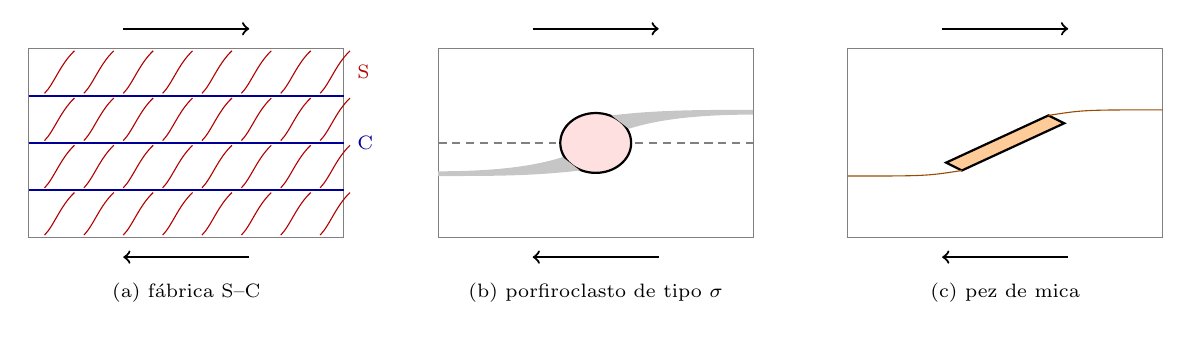
\begin{tikzpicture}[font=\scriptsize, x=1cm, y=1cm]
% (a) S-C fabric, dextral
\begin{scope}
\draw[gray] (0,0) rectangle (4,2.4);
\foreach \y in {0.6,1.2,1.8} {\draw[blue!60!black, thick] (0,\y) -- (4,\y);}
\foreach \y in {0,0.6,1.2,1.8} {\foreach \x in {0.2,0.7,...,3.8} {
  \draw[red!70!black] (\x,\y+0.03) .. controls (\x+0.12,\y+0.15) and (\x+0.2,\y+0.4) .. (\x+0.38,\y+0.57);}}
\draw[->, thick] (1.2,2.65) -- (2.8,2.65);
\draw[<-, thick] (1.2,-0.25) -- (2.8,-0.25);
\node[anchor=north] at (2,-0.45) {(a) fábrica S--C};
\node[blue!60!black, anchor=west] at (4.05,1.2) {C};
\node[red!70!black, anchor=west] at (4.05,2.1) {S};
\end{scope}
% (b) sigma clast
\begin{scope}[shift={(5.2,0)}]
\draw[gray] (0,0) rectangle (4,2.4);
\fill[red!12] (2.0,1.2) ellipse (0.45 and 0.38);
\draw[thick] (2.0,1.2) ellipse (0.45 and 0.38);
\fill[gray!45] (2.2,1.55) .. controls (2.8,1.62) and (3.3,1.62) .. (4.0,1.62) -- (4.0,1.56) .. controls (3.3,1.56) and (2.8,1.5) .. (2.42,1.38) -- cycle;
\fill[gray!45] (1.8,0.85) .. controls (1.2,0.78) and (0.7,0.78) .. (0,0.78) -- (0,0.84) .. controls (0.7,0.84) and (1.2,0.9) .. (1.58,1.02) -- cycle;
\draw[gray, densely dashed] (0,1.2) -- (1.5,1.2) (2.5,1.2) -- (4,1.2);
\draw[->, thick] (1.2,2.65) -- (2.8,2.65);
\draw[<-, thick] (1.2,-0.25) -- (2.8,-0.25);
\node[anchor=north] at (2,-0.45) {(b) porfiroclasto de tipo $\sigma$};
\end{scope}
% (c) mica fish
\begin{scope}[shift={(10.4,0)}]
\draw[gray] (0,0) rectangle (4,2.4);
\fill[orange!40] (1.25,0.95) -- (2.55,1.55) -- (2.75,1.45) -- (1.45,0.85) -- cycle;
\draw[thick] (1.25,0.95) -- (2.55,1.55) -- (2.75,1.45) -- (1.45,0.85) -- cycle;
\draw[orange!60!black] (2.55,1.55) .. controls (3.0,1.62) .. (4.0,1.62);
\draw[orange!60!black] (1.45,0.85) .. controls (1.0,0.78) .. (0,0.78);
\draw[->, thick] (1.2,2.65) -- (2.8,2.65);
\draw[<-, thick] (1.2,-0.25) -- (2.8,-0.25);
\node[anchor=north] at (2,-0.45) {(c) pez de mica};
\end{scope}
\end{tikzpicture}

\par\smallskip{\small Tres \omterm{def:b3:deformation-mechanisms:kinematic}{indicadores cinemáticos} de la misma cizalla dextral
(el techo hacia la derecha, flechas), vistos en el plano de la lineación, normal a la
foliación. (a) La foliación S (roja) se curva hacia las bandas de cizalla C (azules),
inclinándose en la dirección de estiramiento. (b) Las colas de un clasto de tipo $\sigma$
salen de su lado superior hacia la derecha y de su lado inferior hacia la izquierda, escalonándose
en la dirección de cizalla sin cortar la línea central (discontinua). (c) Un
\omterm{def:b3:deformation-mechanisms:kinematic}{pez de mica} se inclina como S, y sus colas escalonan como las de un clasto de tipo $\sigma$. No
está a escala.}\label{fig:b3:deformation-mechanisms:kinematic}
\end{omfigure}

Leídos en conjunto, unos pocos indicadores que coinciden dan el \omterm{def:b3:deformation-mechanisms:kinematic}{sentido de cizalla} con
confianza; uno solo puede inducir a error, ya que existen clastos rotados hacia atrás y
pliegues asimétricos de otro origen. La fotografía del recuadro siguiente muestra
porfiroclastos en una milonita.

\begin{inthelab}[Comprimir roca en condiciones del manto]
\begin{minipage}[t]{0.55\linewidth}\vspace{0pt}
En un aparato de deformación con medio gaseoso, un cilindro de roca o de polvo de olivino
prensado en caliente, de uno o dos centímetros de longitud, se sella en una envoltura metálica delgada y
se coloca con sus pistones dentro de un horno, en una vasija de acero llena de un gas inerte
comprimido que fija la presión de confinamiento, de unos pocos cientos de
megapascales. Un actuador impulsa el pistón a velocidad constante, o bajo una
carga constante, mientras una celda de carga interna mide el esfuerzo sobre la propia muestra,
libre de la fricción de los sellos. El olivino se deforma de este modo a
temperaturas cercanas a \qty{1200}{\celsius}; al final de la prueba la muestra se
enfría bruscamente, se corta, se pule y se examina al microscopio y al
microscopio electrónico, donde se miden su tamaño de grano, sus \omterm{def:b3:deformation-mechanisms:recrystallisation}{subgranos} y sus dislocaciones.
\end{minipage}\hfill
\begin{minipage}[t]{0.42\linewidth}\vspace{0pt}
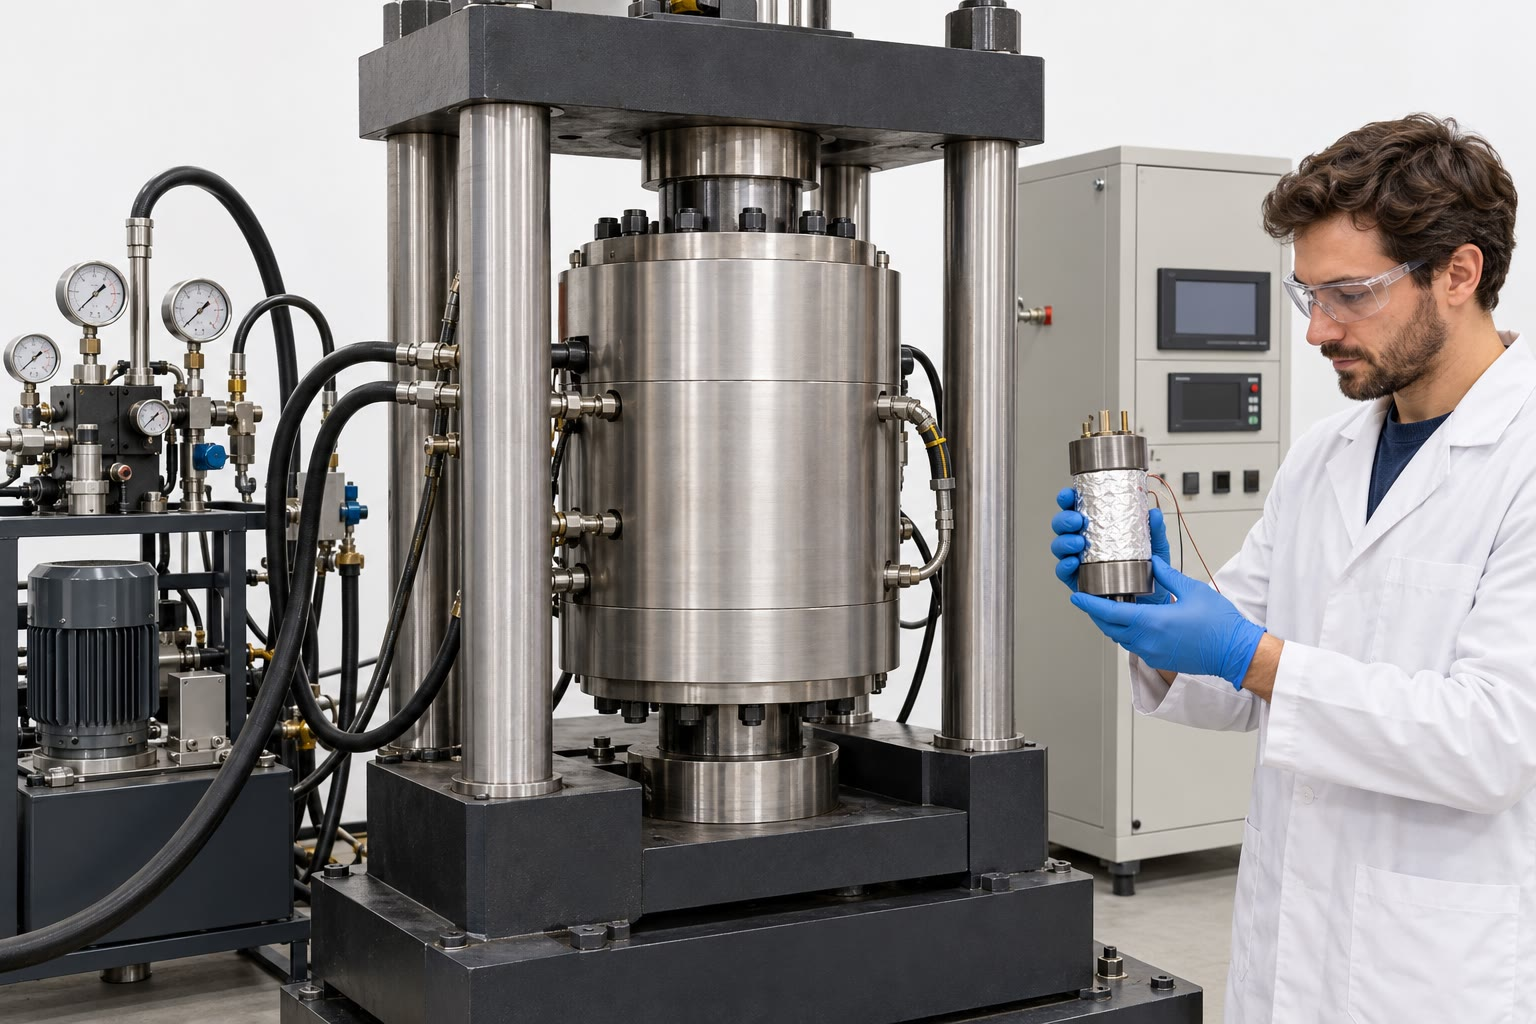
\includegraphics[width=\linewidth]{images/book5/ai/b3-deformation-press.jpg}

{\scriptsize Prensa de deformación de rocas con un conjunto de muestra encamisado
(Ilustración generada por IA).}

\smallskip
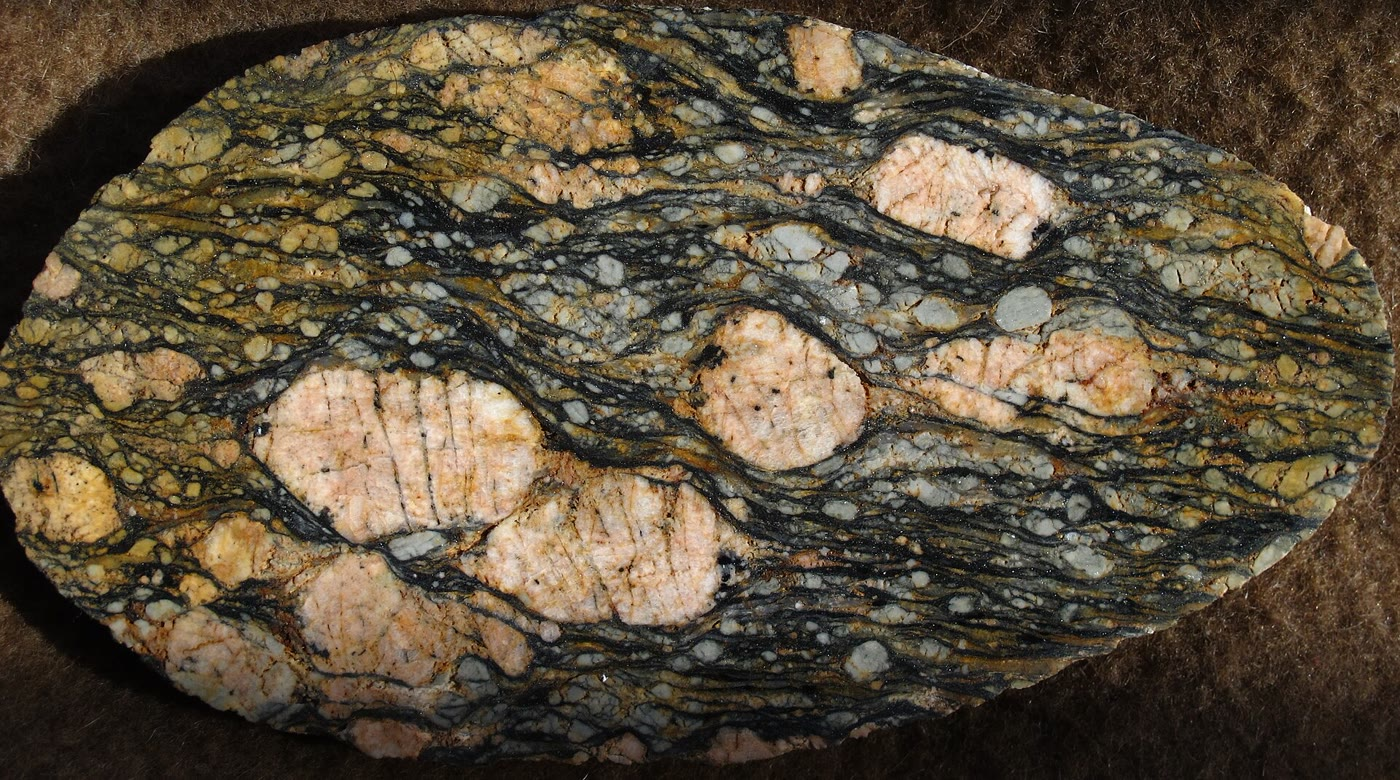
\includegraphics[width=\linewidth]{images/book5/b3-augen-mylonite.jpg}

{\scriptsize Milonita ojosa aserrada procedente de Noruega: grandes porfiroclastos de feldespato
en una matriz fina de cuarzo, feldespato y micas recristalizados. Foto
Mikenorton, CC BY-SA 4.0.}
\end{minipage}
\end{inthelab}
% ledger: mk00:diffusion, photo:b3-augen-mylonite

\section{Ejercicios}

\begin{exercise}[$\star$]\label{exo:b3:deformation-mechanisms:1}
La forsterita funde a \qty{1890}{\celsius} y el hielo a \qty{0}{\celsius}. Calcúlese
la \omterm{def:b3:deformation-mechanisms:flow-law}{temperatura homóloga} de la forsterita a \qty{1300}{\celsius} y la del hielo a
\qty{-10}{\celsius}. ¿Cuál se deforma por fluencia con mayor facilidad?
\end{exercise}

\begin{exercise}[$\star$]\label{exo:b3:deformation-mechanisms:2}
Un dique que atraviesa en ángulo recto una \omterm{def:b3:deformation-mechanisms:shear-zone}{zona de cizalla} se desvía dentro de la
zona \ang{70}, y otro \ang{80}. Calcúlense las deformaciones de cizalla. ¿Por qué las
deformaciones grandes son difíciles de medir de este modo?
\end{exercise}

\begin{exercise}[$\star$]\label{exo:b3:deformation-mechanisms:3}
Con el \omterm{def:b3:deformation-mechanisms:piezometer}{paleopiezómetro} del cuarzo, ¿qué esfuerzo indica un tamaño de grano recristalizado de
\qty{10}{\micro m}?
\end{exercise}

\begin{exercise}[$\star$]\label{exo:b3:deformation-mechanisms:4}
Con la \omterm{def:b3:deformation-mechanisms:flow-law}{ley de flujo} de la cuarcita húmeda ($A = \num{1.1e-4}$, $n = 4$, $E =
\qty{223}{kJ.mol^{-1}}$, $R = \qty{8.314}{J.mol^{-1}.K^{-1}}$), calcúlese la
velocidad de deformación a \qty{500}{\celsius} bajo \qty{20}{MPa}.
\end{exercise}

\begin{exercise}[$\star\star$]\label{exo:b3:deformation-mechanisms:5}
Calcúlese la viscosidad efectiva de la cuarcita húmeda que fluye a \qty{e-14}{s^{-1}}
a \qty{400}{\celsius} (\qty{65.4}{MPa}) y a \qty{500}{\celsius}
(\qty{18.0}{MPa}). Compárense con las \omterm{def:b3:mantle-convection:gia}{viscosidades del manto}
descritas en el \cref{ch:b3:mantle-convection}.
\end{exercise}

\begin{exercise}[$\star\star$]\label{exo:b3:deformation-mechanisms:6}
Dos experimentos a la misma temperatura dan \qty{e-5}{s^{-1}} bajo
\qty{100}{MPa} y \qty{1.6e-4}{s^{-1}} bajo \qty{200}{MPa}. Calcúlese el \omterm{def:b3:deformation-mechanisms:flow-law}{exponente
de esfuerzo} e indíquese el mecanismo probable.
\end{exercise}

\begin{exercise}[$\star\star$]\label{exo:b3:deformation-mechanisms:7}
Al mismo esfuerzo, una muestra se deforma por fluencia diez veces más rápido a
\qty{1100}{K} que a \qty{1000}{K}. Calcúlese la energía de activación.
\end{exercise}

\begin{exercise}[$\star\star$]\label{exo:b3:deformation-mechanisms:8}
¿En qué factor cambia la velocidad de deformación por \omterm{def:b3:deformation-mechanisms:creep}{fluencia por difusión} cuando el
tamaño de grano se divide por diez, para la fluencia de Nabarro--Herring y la de Coble?
¿Por qué la fluencia de Coble es la más sensible?
\end{exercise}

\begin{exercise}[$\star\star$]\label{exo:b3:deformation-mechanisms:9}
Para olivino seco a \qty{1100}{\celsius} y \qty{2}{GPa}, las dos \omterm{def:b3:deformation-mechanisms:flow-law}{leyes de flujo} dan
$\dot\varepsilon_{\mathrm{dis}} = \num{6.54e-17}\,\sigma^{3.5}$ y
$\dot\varepsilon_{\mathrm{dif}} = \num{3.59e-6}\,\sigma d^{-3}$ (unidades del
texto). Calcúlese el esfuerzo de transición para $d = \qty{1}{mm}$ y $d =
\qty{100}{\micro m}$, y la pendiente de la línea de transición.
\end{exercise}

\begin{exercise}[$\star\star\star$]\label{exo:b3:deformation-mechanisms:10}
Siguiendo la demostración de la \cref{prop:b3:deformation-mechanisms:grain-size},
explíquese por qué la trayectoria por red da $d^{-2}$ y la trayectoria por frontera $d^{-3}$, y
muéstrese que la difusión por borde de grano domina por debajo del tamaño de grano $d^* \approx
(B_B/B_L)\,\delta D_B/D_L$.
\end{exercise}

\begin{exercise}[$\star\star\star$]\label{exo:b3:deformation-mechanisms:11}
Para una \omterm{def:b3:deformation-mechanisms:flow-law}{ley de flujo} con $n = 3.5$, ¿en qué factor disminuye la viscosidad efectiva
cuando la velocidad de deformación se multiplica por diez? ¿Por qué esto favorece la
localización de la deformación en \omterm{def:b3:deformation-mechanisms:shear-zone}{zonas de cizalla}?
\end{exercise}

\begin{exercise}[$\star\star\star$]\label{exo:b3:deformation-mechanisms:12}
En el olivino seco del ejercicio 9, una \omterm{def:b3:deformation-mechanisms:shear-zone}{zona de cizalla} del manto bajo \qty{10}{MPa}
se recristaliza de granos de \qty{3}{mm} a granos de \qty{30}{\micro m}. Calcúlese la
velocidad de deformación total antes y después, y el factor de debilitamiento. ¿Qué
mecanismo transporta la deformación en cada caso?
\end{exercise}

\section{Problema: la zona de cizalla de Varden}

\begin{problem}[{Problema de fin de semana --- la deformación, el esfuerzo, la velocidad de
deformación y la edad de una zona de cizalla inventada}]
\label{pb:b3:deformation-mechanisms:1}
% values: calc/ch07.py; flow_laws.py; st03:piezometer, lopez:flow-laws
Bajo el granito de las colinas de Varden, la región inventada de la serie, un sondeo y
un corte profundo de carretera (ambos inventados) revelan una \omterm{def:b3:deformation-mechanisms:shear-zone}{zona de cizalla} dúctil de
\qty{400}{m} de anchura, formada a unos \qty{15}{km} de profundidad y \qty{450}{\celsius}.
Un dique de dolerita que atraviesa las paredes en ángulo recto forma, dentro de la zona,
un ángulo de solo \ang{6} con los límites de la zona. Su cuarzo es una milonita de granos
recristalizados de \qty{20}{\micro m} de diámetro (de 15 a
\qty{25}{\micro m}). Tómense el \omterm{def:b3:deformation-mechanisms:piezometer}{paleopiezómetro} del cuarzo $D = 10^{3.56}\sigma^{-1.26}$,
la \omterm{def:b3:deformation-mechanisms:flow-law}{ley de flujo} de la cuarcita húmeda ($A = \num{1.1e-4}$, $n = 4$, $E =
\qty{223}{kJ.mol^{-1}}$), $R = \qty{8.314}{J.mol^{-1}.K^{-1}}$, \qty{1}{yr} $=
\qty{3.156e7}{s}$, y, en cizalla simple, $\dot\gamma = 2\dot\varepsilon$.

\medskip\noindent\textbf{Parte I --- La deformación.}
\begin{enumerate}
  \item Calcúlese la deflexión $\psi$ del dique y la deformación de cizalla.
  \item Calcúlese el desplazamiento de una pared respecto de la otra.
  \item Calcúlense los estiramientos principales de la elipse de deformación y su
        razón axial.
  \item Calcúlese el ángulo del eje largo con la zona. ¿Qué hace la
        foliación de la zona a medida que crece $\gamma$?
  \item Vista desde arriba, el dique, seguido desde la pared sur, se curva hacia el
        este al entrar en la zona de dirección este--oeste, luego recupera su
        rumbo hacia el norte en la pared norte. ¿Hacia qué lado se movió la
        pared norte, y es la zona dextrógira o levógira?
  \item ¿En qué plano debe cortarse una lámina delgada para leer los \omterm{def:b3:deformation-mechanisms:kinematic}{indicadores
        cinemáticos}, y cómo debe inclinarse su foliación S?
\end{enumerate}

\medskip\noindent\textbf{Parte II --- El esfuerzo.}
\begin{enumerate}[resume]
  \item Calcúlese el esfuerzo que indican los granos de \qty{20}{\micro m}.
  \item Calcúlense los esfuerzos para 15 y \qty{25}{\micro m}.
  \item ¿Está el esfuerzo dentro del intervalo de calibración?
  \item El \omterm{def:b3:deformation-mechanisms:piezometer}{paleopiezómetro} no mostró efecto de la temperatura. ¿Por qué importa
        esto aquí?
  \item ¿Qué tamaño de grano habría producido un esfuerzo de \qty{100}{MPa}?
\end{enumerate}

\medskip\noindent\textbf{Parte III --- La velocidad de deformación.}
\begin{enumerate}[resume]
  \item Calcúlense $E/RT$ a \qty{450}{\celsius} y el factor de Arrhenius.
  \item Calcúlese la velocidad de deformación del cuarzo bajo el esfuerzo de la pregunta 7
        (tómense \qty{62}{MPa}).
  \item Calcúlese la velocidad de deformación de cizalla.
  \item Calcúlese la viscosidad efectiva de la zona y compárese con el
        manto superior del \cref{ch:b3:mantle-convection}.
  \item ¿En qué factores cambiaría la velocidad de deformación a 400 y
        \qty{500}{\celsius}, con el mismo esfuerzo?
  \item ¿En qué factor cambiaría si el esfuerzo fuera el de \qty{78}{MPa} de los
        granos más finos?
\end{enumerate}

\medskip\noindent\textbf{Parte IV --- El tiempo.}
\begin{enumerate}[resume]
  \item Calcúlese el tiempo necesario para acumular la deformación de cizalla de la pregunta 1,
        en segundos.
  \item Conviértase en miles de años.
  \item Calcúlese la velocidad media de deslizamiento a través de la zona, en \unit{mm/yr}.
  \item Compárese con las velocidades de límite de placa de decenas de milímetros al año.
        % ledger: morvel:range
  \item Si la zona hubiera transportado \qty{20}{mm/yr}, ¿qué velocidad de deformación de cizalla, esfuerzo
        y tamaño de grano recristalizado habría tenido?
  \item ¿Cómo afectan las incertidumbres del tamaño de grano y del exponente del
        piezómetro al tiempo?
  \item Indíquese el tiempo que tardó la \omterm{def:b3:deformation-mechanisms:shear-zone}{zona de cizalla} de Varden en acumular su deformación, en
        miles de años.
\end{enumerate}
\end{problem}
